\documentclass[article, paper=a4, fleqn, fontsize=10.5bp, line_length=40zw, gutter=30mm, head_space=35mm, foot_space=30mm]{jlreq}

\usepackage{ifluatex}
\ifluatex
    \usepackage{graphicx, xcolor}
    \usepackage{luatexja-otf}
    % \usepackage{luatexja-fontspec}
    % \usepackage[ms]{luatexja-preset}
    % \setmainfont[Ligatures=TeX]{Times New Roman}
\else
    \usepackage[dvipdfmx]{graphicx, xcolor}
\fi
\usepackage[intlimits]{amsmath}
\usepackage{newtxtext, newtxmath}

\usepackage{mathrsfs}  % \mathscr用
\usepackage{booktabs}  % 綺麗な表組み
\usepackage{multirow}  % 複数行や複数列に跨る表組み
\usepackage{type1cm}  % フォント拡大縮小
\usepackage{scalefnt}  % フォント拡大縮小
\usepackage{comment}  % 複数行のコメントアウト
\usepackage{subfigure}  % 図を複数並べる

% Citation form
\makeatletter
  \def\@biblabel#1{(#1)}
\makeatother
\usepackage{overcite}
\renewcommand\citeform[1]{(#1)}

% Caption
\renewcommand{\figurename}{Fig.~}  % 図 -> Fig.
\renewcommand{\tablename}{Table~}  % 表 -> Table

% 文書
\begin{document}

\pagestyle{empty}

% Title
\begin{center}
{\scalefont{2} \textgt{計画書}}
\end{center}
\vspace{0.3cm}
\begin{flushright}
{20XX年XX月XX日作成}
\\
{〇〇 〇〇}
\end{flushright}

% 本文
\section{研究題目}
〇〇〇〇〇〇〇〇

\section{研究背景}
Burgersベクトルは,現配置において式~\eqref{eq_bergers_vector}で表される~\cite{kondo1955non-riemannian}.
%
\begin{equation}
    \label{eq_bergers_vector}
    \tilde{B}{}^{a}
    = -\int_{\mathscr{S}} \left[ \hat{T}{}^{..a}_{bc} + \frac{1}{2} C^{\ell{}-1ae} \left( \hat{R}{}_{bc[de]} + \hat{R}{}_{bc(de)} \right) x^{d} \right] \mathrm{d} x^{b} \wedge \mathrm{d} x^{c}
    \dotfill
\end{equation}
%
これを図示すると,図~\ref{fig_paper_irasutoya}のようになる.
%
\begin{figure}[bp]
    \centering
    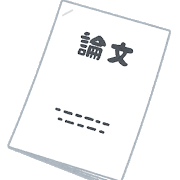
\includegraphics{./figure/document_ronbun_taba.png}
    \caption{Paper.}
    \label{fig_paper_irasutoya}
\end{figure}
%

% 参考文献
\bibliographystyle{./chap/sjunsrt_d.bst}
\bibliography{./chap/reference.bib}

\end{document}
